\documentclass[11pt,a4paper]{article}
\usepackage[utf8]{inputenc}
\usepackage[T1]{fontenc}

\usepackage[margin=2cm]{geometry}
\usepackage{xcolor}
\usepackage{enumitem}
\usepackage{booktabs}
\usepackage{tabularx}
\usepackage{fancyhdr}
\usepackage{titlesec}
\usepackage{parskip}
\usepackage{hyperref}
\usepackage{tcolorbox}
\tcbuselibrary{skins,breakable}
\usepackage{tikz}
\usetikzlibrary{positioning}
\usepackage{multicol}

\definecolor{accent}{HTML}{0f3460}
\definecolor{dark}{HTML}{1a1a2e}
\definecolor{highlight}{HTML}{e94560}
\definecolor{softblue}{HTML}{e8f0fe}
\definecolor{softgreen}{HTML}{e8f5e9}
\definecolor{midgray}{HTML}{666666}

\hypersetup{colorlinks=true,linkcolor=accent,urlcolor=accent}

\titleformat{\section}{\Large\bfseries\color{accent}}{}{0em}{}[\vspace{-0.5em}\textcolor{accent}{\rule{\textwidth}{0.6pt}}]
\titleformat{\subsection}{\large\bfseries\color{dark}}{}{0em}{}

\pagestyle{fancy}
\fancyhf{}
\fancyhead[L]{\small\textcolor{gray}{XC Gradient --- Equip Fundador}}
\fancyhead[R]{\small\textcolor{gray}{Confidencial}}
\fancyfoot[C]{\small\textcolor{gray}{\thepage}}
\renewcommand{\headrulewidth}{0.4pt}

\newtcolorbox{profilebox}[1][]{
  colback=softblue,colframe=accent,
  boxrule=0.5pt,left=8pt,right=8pt,top=6pt,bottom=6pt,
  breakable,#1
}

\newtcolorbox{skillbox}[1][]{
  colback=white,colframe=midgray,
  boxrule=0.3pt,left=4pt,right=4pt,top=3pt,bottom=3pt,#1
}

\begin{document}

\begin{center}
{\Huge\bfseries\color{dark} Equip Fundador}\\[0.3em]
{\Large\color{accent} XC Gradient}\\[0.5em]
{\small\color{midgray} Abril 2026 $\cdot$ Confidencial}
\end{center}

\vspace{0.5em}
{\color{accent}\hrule height 1pt}
\vspace{0.5em}

\begin{center}
\colorbox{softgreen}{\parbox{0.85\textwidth}{\centering\small
Tres enginyers informàtics per la UPC-FIB (Facultat d'Informàtica de Barcelona), amb cobertura completa de les tres capes crítiques del producte: IA/ML, infraestructura de dades i ciberseguretat. Equity igualitari (1/3 cada un).
}}
\end{center}

\vspace{1em}

%% ─── ORIOL ─────────────────────────────────────

\begin{profilebox}[title={\large\bfseries\color{dark} Oriol Farrés i Vilar \hfill \normalsize CEO / CFO}]

\begin{minipage}[t]{0.65\textwidth}
\textbf{Formació}\\
Grau en Enginyeria Informàtica --- UPC-FIB, Barcelona\\
Màster en Enginyeria Informàtica --- UPC-FIB (en curs, defensa: juliol 2026)\\
\small Tesi: \textit{``The Post-Retrieval Markov Chain: Optimizing Information Flow through Game-Theoretic Compression and Role-Conditioned Alignment''}\\
Supervisor: Dr. Lluís Padró

\vspace{0.5em}
\textbf{Rol a XC Gradient}\\
Arquitectura core d'IA i pipeline IP tesi$\rightarrow$producte. Lidera estratègia de negoci, relacions amb clients, product-market fit i projecció financera.
\end{minipage}%
\hfill%
\begin{minipage}[t]{0.32\textwidth}
\small
\textbf{Àrees de propietat IP}
\begin{itemize}[leftmargin=0.8em,itemsep=1pt,topsep=2pt]
\item Reranking Markov+Choquet
\item Fine-tuning S-QDoRA
\item Speculative decoding
\item Framework d'avaluació (ensemble 7-features)
\end{itemize}
\end{minipage}

\vspace{0.5em}
\begin{skillbox}
\small\textbf{Competències clau:} Arquitectura de sistemes d'IA $\cdot$ Teoria de jocs aplicada $\cdot$ Optimització d'inferència $\cdot$ Estratègia de negoci $\cdot$ Relació amb clients industrials $\cdot$ Planificació financera
\end{skillbox}

\vspace{0.3em}
\small\textbf{Contribucions destacades:}
\begin{itemize}[leftmargin=1.2em,itemsep=1pt]
\item Formalització del pipeline RAG com a cadena de Markov absorbent amb reranking per integral de Choquet --- supera les limitacions dels mètodes de scoring additiu capturant sinergies entre chunks documentals.
\item Disseny de S-QDoRA: mètode de fine-tuning multi-tenant que permet especialització per client amb adaptadors dispersos sobre model base quantitzat --- eliminant la necessitat d'un model complet per client.
\item Disseny del framework de benchmarking que substitueix RAGAS amb un ensemble calibrat contra anotacions humanes, amb protocol estadístic pre-registrat.
\item Lideratge del pivot estratègic del pitch de Paver: reorientació de ``manteniment predictiu'' cap a ``recuperació de coneixement'' basant-se en l'objecció de variabilitat de matrius del CEO.
\end{itemize}
\end{profilebox}

\vspace{1em}

%% ─── ARNAU ─────────────────────────────────────

\begin{profilebox}[title={\large\bfseries\color{dark} Arnau Noguer \hfill \normalsize CTO / AI}]

\begin{minipage}[t]{0.65\textwidth}
\textbf{Formació}\\
Grau en Enginyeria Informàtica --- UPC-FIB, Barcelona

\vspace{0.5em}
\textbf{Rol a XC Gradient}\\
Propietari del motor RAG complet: des de la ingestió de documents fins a la recuperació, i la capa d'ontologia que fa el sistema conscient del domini manufacturerer.
\end{minipage}%
\hfill%
\begin{minipage}[t]{0.32\textwidth}
\small
\textbf{Àrees de propietat}
\begin{itemize}[leftmargin=0.8em,itemsep=1pt,topsep=2pt]
\item Pipeline d'ingestió
\item Motor de recuperació híbrid
\item Ontologies per client
\item Vector store aïllat
\end{itemize}
\end{minipage}

\vspace{0.5em}
\begin{skillbox}
\small\textbf{Competències clau:} Sistemes RAG $\cdot$ Processament de llenguatge natural $\cdot$ Infraestructura LLM $\cdot$ Enginyeria de dades $\cdot$ Cerca híbrida densa+dispersa $\cdot$ Construcció d'ontologies
\end{skillbox}

\vspace{0.3em}
\small\textbf{Responsabilitats actuals:}
\begin{itemize}[leftmargin=1.2em,itemsep=1pt]
\item Pipeline RAG sobre corpus de Decfa: ingestió de documentació tècnica, manuals de maquinària, i registres de manteniment CNC.
\item Objectiu d'A-score $>$0.80 al framework d'avaluació (target: 15 maig 2026).
\item Configuració d'infraestructura d'inferència LLM.
\item Runbook de desplegament per a clients (target: maig 2026).
\end{itemize}
\end{profilebox}

\vspace{1em}

%% ─── ADAM ─────────────────────────────────────

\begin{profilebox}[title={\large\bfseries\color{dark} Adam Sarrate \hfill \normalsize COO / CISO}]

\begin{minipage}[t]{0.65\textwidth}
\textbf{Formació}\\
Grau en Enginyeria Informàtica --- UPC-FIB, Barcelona

\vspace{0.5em}
\textbf{Rol a XC Gradient}\\
Propietari de la topologia de desplegament i l'arquitectura de seguretat que defineix com les dades es mouen pel sistema. Responsable d'operacions i conformitat regulatòria.
\end{minipage}%
\hfill%
\begin{minipage}[t]{0.32\textwidth}
\small
\textbf{Àrees de propietat}
\begin{itemize}[leftmargin=0.8em,itemsep=1pt,topsep=2pt]
\item Topologia de xarxa
\item Arquitectura de seguretat
\item Desplegament on-premises
\item Documentació de conformitat
\end{itemize}
\end{minipage}

\vspace{0.5em}
\begin{skillbox}
\small\textbf{Competències clau:} Ciberseguretat $\cdot$ Arquitectura de xarxa $\cdot$ NIS2 / ISO~27001 $\cdot$ Desplegament on-premises $\cdot$ Control d'accés $\cdot$ Operacions
\end{skillbox}

\vspace{0.3em}
\small\textbf{Responsabilitats actuals:}
\begin{itemize}[leftmargin=1.2em,itemsep=1pt]
\item Disseny del graf de topologia de xarxa per a desplegaments a plantes industrials.
\item Definició de garanties d'aïllament entre clients, control d'accés al contenidor privat, i model de flux de dades.
\item Documentació de seguretat orientada a client (què recollim, com s'emmagatzema, qui hi pot accedir).
\item Runbook de desplegament segur on-premises.
\end{itemize}
\end{profilebox}

\vspace{1.5em}

\section{Cobertura de l'Equip}

\begin{center}
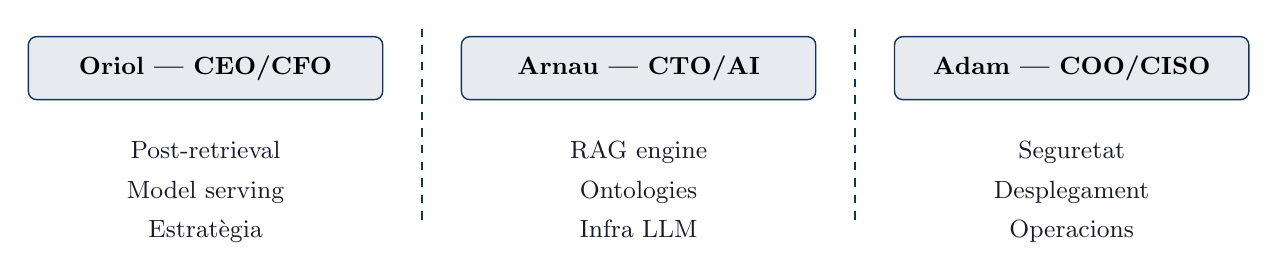
\begin{tikzpicture}[
  block/.style={rectangle, rounded corners=3pt, draw=#1, fill=#1!10,
    minimum width=4.5cm, minimum height=0.8cm, align=center,
    font=\small\bfseries, line width=0.5pt},
  label/.style={font=\small\color{dark}}
]

\node[block=accent] (oriol) at (0,0) {Oriol --- CEO/CFO};
\node[block=accent] (arnau) at (5.5,0) {Arnau --- CTO/AI};
\node[block=accent] (adam) at (11,0) {Adam --- COO/CISO};

\node[label, below=0.4cm of oriol] {Post-retrieval};
\node[label, below=0.9cm of oriol] {Model serving};
\node[label, below=1.4cm of oriol] {Estratègia};

\node[label, below=0.4cm of arnau] {RAG engine};
\node[label, below=0.9cm of arnau] {Ontologies};
\node[label, below=1.4cm of arnau] {Infra LLM};

\node[label, below=0.4cm of adam] {Seguretat};
\node[label, below=0.9cm of adam] {Desplegament};
\node[label, below=1.4cm of adam] {Operacions};

\draw[thick, accent, dashed] (2.75, 0.5) -- (2.75, -2);
\draw[thick, accent, dashed] (8.25, 0.5) -- (8.25, -2);

\end{tikzpicture}
\end{center}

\vspace{0.5em}
\begin{center}
\small\textcolor{midgray}{L'equip cobreix les tres capes crítiques: intel·ligència artificial, dades/retrieval i seguretat/operacions.\\
Cap dependència externa per al desenvolupament core del producte.}
\end{center}

\vfill
\begin{center}
\small\textcolor{midgray}{XC Gradient $\cdot$ Equip Fundador $\cdot$ Confidencial $\cdot$ Abril 2026}
\end{center}

\end{document}
